\section{Zielsetzung}

Der vorliegende Versuch behandelt die Ermittlung der Lebensdauer
kosmischer Myonen. Zu Beginn wird in die Theorie des Versuches eingeleitet.
Anschließend wird die Messapparatur und die Durchführung der Messung beschrieben.
Abschließend werden die gemessenen Ergebnisse ausgewertet und abschließend diskutiert.

\section{Theorie}

Myonen $\mu$ sind Leptonen der zweiten Generation und besitzen eine Masse
von $\approx \SI{106}{\mega\eV}$.
Sie entstehen zum Großteil in der oberen Atmosphäre durch Pion-Zerfälle und
besitzen resultierend aus dem Zerfall, eine hohe kinetische Energie.

\begin{align}
  \label{eqn:pion+ nach myon}
  \ce{\pi^+ &-> \mu^+ + \nu\ua{\mu}}\\
  \label{eqn:pion- nach myon}
  \ce{\pi^- &-> \mu^- + \bar{\nu}\ua{\mu}}
\end{align}

Myonen sind ca. 207 mal so schwer wie Elektronen.
Myonen zerfallen nach den folgenden Zerfallsgleichungen.

\begin{align}
  \label{eqn:myon+ nach e+}
  \ce{\mu^+ &-> \symup{e}^+ + \nu\ua{e} + \bar{\nu}\ua{\mu}}\\
  \label{eqn:moyn- nach e-}
  \ce{\mu^- &-> \symup{e}^- + \bar{\nu}\ua{e} + \nu\ua{\mu}}
\end{align}

\subsection{Lebensdauer}

Die Lebensdauer $\tau$ eines instabilen Teilchens beschreibt die Zeit,
nach der eine Teilchenpopulation auf $\frac{1}{\symup{e}}$ ihrer ursprünglichen
Anzahl abgefallen ist.
Der Zerfall eines Teilchens ist ein stochastischer Prozess, der durch
ein Exponentialgesetz der Form:

\begin{equation}
  \label{eqn:Lebensdauer}
  N(t) = N_0\cdot\exp{\left(-\frac{t}{\tau}\right)}
\end{equation}

beschrieben wird. Die Zerfallskonstante $\lambda$ entspricht der reziproken
Lebensdauer.

Die Funktion \ref{eqn:Lebensdauer} ist die Lösung der folgenden Differentailgleichung.

\begin{equation}
  \label{eqn:herleitung_lebensdauer}
  \frac{\symup{d}N}{\symup{d}t} = -\lamdba\cdot N
\end{equation}

Dabei wird angesetzt, dass die Anzahl der Teilchen $N$ pro Zeit $t$
proportional zu der Zerfallskosntante $\lambda$ ist. Das Vorzeichen erklärt sich dadurch,
dass die Anzahl aufgrund des Zerfallsprozesses mit der Zeit abnimmt.

\section{Versuchsaufbau}

Damit die Lebensdauer von Myonen bestimmt werden kann, dürfen nur
Myonen gemessen werden, von denen die Einlaufzeit in den Versuchsaufbau bekannt ist
und weiterhin deren Zerfallszeit nach eindringen gemessen wurde.
Somit sind nur Myonen, die auch in dem Versuchsaufbau zerfallen relevant
für die Messung. Im Folgenden wird der verwendete Versuchsaufbau beschrieben,
der das Herausfiltern dieser relevanten Ereignisse ermöglicht.

Grundlegend wird für die Detektion von Teilchen ein Szintillator verwendet.
Ionisierende Teilchen, die den Szintillator durchqueren, wechselwirken mit den Atomen
des Szintillatormaterials. Durch diese Wechselwirkung können
die Atome im Szintillator in einen angeregten Zustand überführt werden.
Myonen haben eine hohe kinetische Energie und können mehrere MeV ihrer kinetischen Energie
an das Szintillatormaterial abgeben. Die angeregten Szintillatoratome geben
bei dem Übergang von dem angeregten Zustand in den Grundzustand einen Lichtquant
ab, der von einer optisch an den Szintillator gekoppelten Photokathode
registriert werden kann.
An der Photokathode liegt ein sekundärer Elektronenvervielfältiger (SEV) an.
Der SEV verstärkt die Signale aus der Photokathode, damit sie detektiert werden
können.

Das Filtern der Ereignisse von Myonen, die auch in dem Szintillator zerfallen,
geschieht durch eine logische Schaltung. Diese Schaltung ist in Abb. \ref{fig:Aufbau}
durch die beiden AND-Gatter und den Monoflop/Univibrator realisiert.
Anliegende Spannungen werden im Folgenden als HIGH und das Fehlen von Spannungen
als LOW bezeichnet.
Wenn ein HIGH aus der Koinzidenz (vgl. Abb. \ref{fig:Aufbau}), deren Funktion im
Verlauf der Durchfürhung noch erklärt wird, in die untere Schaltung einläuft
wird zunächst der rechte Eingang des 1. und 2. UND-Gatter auf HIGH gesetzt.
Das aus der Koinzidenz stammende
HIGH wird mit einer Verzögerung von $\SI{30}{\nano\second}$ an den Univibrator
abgegeben. An dem einen Ausgang des Univibrators, der mit dem 1. UND verbunden
ist, liegt im LOW Zustand ein HIGH an (vgl. Abb. \ref{fig:Aufbau}; $\bar{\text{OUT}}$).
Der zweite Ausgang ist mit dem 2. UND verbunden
und gibt im LOW Zustand des Univibrators ein LOW weiter (OUT).
Somit sind an dem 1. UND beide Eingänge mit einem HIGH belegt und das Startsignal wird
an einen Zeit-Amplituden-Konverter und Impulszähler gegeben. Der Impulszähler
zählt lediglich die Anzahl der eintreffenden Startsignale.
Der Zeit-Amplituden-Konverter wandelt die vergehende Zeit zwischen einem
HIGH an dem Starteingang und einem HIGH an dem Stoppeingang in eine
dazu proportionalen Impuls. Die Zeit wird in der Höhe des Impulses
kodiert.
Ein einlaufendes HIGH in den Univibrator kehrt die HIGH und LOW Signale an
den Ausgängen um.
Nach einer einegstellten Zeit $T\ua{s}$ geht der Monoflop in seinen Grundzustand
zurück. $T\ua{s}$ stellt die Suchzeit des Intervalls einer Myonenlebensdauermessung
dar. In dem Versuch wird $T\ua{s} = \SI{10}{\micro\second}$ gewählt.
Der linke Eingang des 2. UND-Gatters empfängt, nachdem
der Monoflop ein HIGH erhalten hat, ebenfalls ein HIGH, welches für
die eingestellte Zeit $T\ua{s}$ anliegt. Wird in diesem
Zeitraum ein weiteres Signal von der Koinzidenz an den rechten Eingang des
2. UND-Gatters geleitet wird ein HIGH an den Stoppeingang des Zeit-Impuls-Konverters gegeben
und die Zeitmessung ist abgeschlossen. Die in einem Impuls kodierte Zerfallszeit
wird in ein Vielkanalanalysator gegeben, welcher mit einem Computer
verbunden ist. Der Rechner verarbeitet das Signal mit geeigneter Software.

In dem Versuch sollen nur die durch Myonen erzeugten Ereignisse behandelt werden.
Jedoch werden durch thermische Prozesse in dem Photkathoden statischtisch verteilt
Elektronen gelöst, welche von den SEV als Myonenereignisse interpretiert werden.
Um dieses thermische Rauschen zu unterdrücken gibt es zwei parallel angewendete
Mechanismen. Die thermischen Störungen lösen in der Regel eine niederigere
Spannung als die Myonenereignisse aus, je nachdem an welcher Dynode des Photomultipliers
das Elektron ausgelöst wird. Durch einen Diskriminator werden nur
Ereignisse durchgelassen, die einen einstellbaren Schwellenwert $U_0$ übersteigen.
Damit können thermische Ereignisse signifikant unterdrückt werden.
Zudem werden die Ereignisse die den Schwellenwert des Diskriminatros übersteigen
mit einheitlicher Spannungsamplitude weitergeleitet.
Vor den Diskriminatoren sind Verzögerungen angebracht, damit Materialeigenschaften
der Diskriminatoren kompensiert werden können.

Der zweite rauschunterdrückende Mechanismus ist die Koinzidenz.
Diese lässt nur nahezu gleichzeitig einlaufende Signale passieren.
Die einlaufenden Signale dürfen einen Zeitversatz von $\Delta t\ua{k}\approx
\SI{4}{\nano\second}$ besitzen.
Die thermisch gelösten Elektronen entstehen in einer Phtotkathode bzw. SEV, somit gibt
es in der Regel kein zeitgleiches Signal des anderen SEV. So kann das
thermische Rauschen mithilfe der Koinzidenz ebenfalls unterdrückt werden.
%nd sind deutlich langsamer als durch Myonen entstehende Ereignisse und
%erreichen die Koinzidenz mit einer geringen Wahrscheinlichkeit in dem
%Zeitintervall $\Delta t\ua{k}$.




\begin{figure}[h]
  \centering
  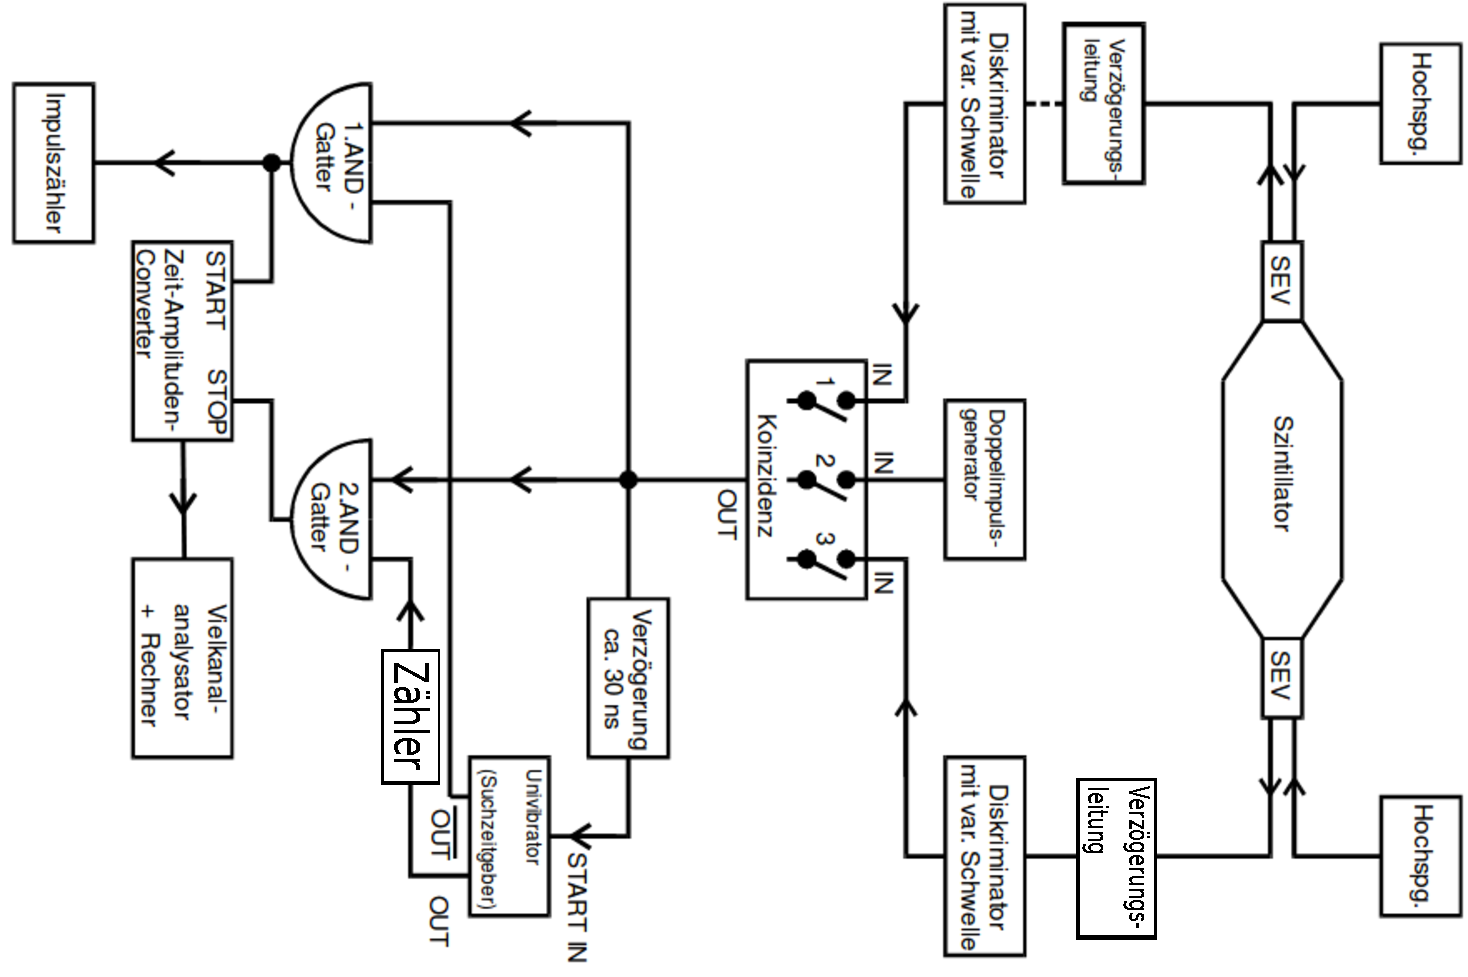
\includegraphics[width=\textwidth, angle=90]{Pics/Aufbau_angepasst.pdf}
  \caption{Schematischer Versuchsaufbau \cite{anleitung01}}
  \label{fig:Aufbau}
\end{figure}

Der Versuch wird mit dem Aufbau aus Abb. \ref{fig:Aufbau} durchgeführt. In
dem realen Aufbau ist ein weiterer Verzögerer vor dem rechten Diskriminator angebracht,
sodass eine Verzögerung der beiden Messkanäle relativ zu einander eingestellt werden kann.

Der in Abb. \ref{fig:Aufbau} dargestellte Doppelimpulsgenerator wird
für die Kalibration des Vielkanalanalysators verwendet, worauf in der
Durchführung näher eingegangen wird.

Es wird ein organischer Szintillator verwendet, da dieser
im Vergleich zu einem anorganischen Szintillator eine kürzere
Totzeit besitzt. Insgesamt fasst der Szintillatortank 50l und ist in Toluol gelöst.

\subsection{Durchführung}

Zu Beginn des Versuches wird der Versuchsaufbau gemäß Abb. \ref{fig:Aufbau} aufgebaut.
Dabei wird der Aufbau während des Aufbauens mit einem Zwei-Kanal-Oszilloskop
auf seine Funktionsfähigkeit überprüft werden.
Die Schwellenwerte $U_0$ der Diskriminatoren werden so eingestellt, dass
die Impulsrate aus beiden Kanälen ungefähr übereinstimmt. Für das Zählen der
Impulsrate werden die Messkanäle an den Impulszähler angeschlossen.
Die Impulsrate sollte zwischen 20 und 40 Impulsen pro Sekunde liegen.
Falls der aufgenommene Wert nicht in diesem Intervall liegt, kann die
Schewellenspannung $U_0$ variiert werden, bis die Impulsrate den Anforderungen genügt.

Weiterhin gilt es, die Verzögerer die vor dem Diskriminatoren montiert sind
abzugleichen, sodass die materialbedingte Verzögerung der beiden Messkanäle
kompensiert wird. Dies ist essentiell für die Arbeitsweise der Koinzidenz.
Dafür werden jeweils fünf Messwerte für die Einstellungsmöglichkeit der Verzögerer genommen.
Währenddessen wird die Impulsrate mittels des angeschlossenen Impulszählers, welcher hinter
der Koinzidenz liegt aufgenommen.
Die Verzögerung, bei der die Impulsrate maximal ist, ist die von nun an einzustellende.

Die Koinzidenzapparatur kann durch Vergleich der vor und hinter der Koinzidenz
registrierten Impulse überprüft werden. Stimmen beide Werte überein ist
die Funktion als Rauschunterdrücker nicht gewährleistet und die Einstellungen müssen
verändert werden.

Der Zeit-Amplituden-Konverter kann überprüft werden, indem vor die Koinzidenz ein
Doppelimpulsgenerator geschaltet wird. Der zeitliche Abstand der
Doppelimpulse kann in Stufen von $0,1\si{\micro\second}$ variiert werden.
Die Funktionsfähigkeit des Doppelimpulsgenerators kann mit Hilfe des
Zwei-Kanal-Oszilloskopen überprüft werden.
Der Zeit-Amplituden-Konverter arbeitet einwandfrei, wenn an seinem
Ausgang Spannungsimpulse entstehen, die proportional zu der
eingestellten Zeit des Doppelimpulsgenerators sind. Mit dem Zwei-Kanal-Oszilloskop
ist die Arbeitsfähigkeit des Zeit-Amplituden-Konverters zu überprüfen.

Der Vielkanalanalysator wird justiert durch eine Kalibirerungsmessung.
Dafür werden mit dem Doppelimpulsgenerator Spannungsimpulse erzeugt.
Es werden soviele Werte aufgenommen, bis sich auf dem Rechner deutlich
erkennbare Balken in den Kanälen entstanden sind.
Die Zeit der aufeinanderfolgenden Doppelimpulse wird in Schritten von $\SI{1}{\micro\second}$
erhöht von 0 bis auf $\SI{9.9}{\micro\second}$.

Abschließend wird die Messapparatur für insgesamt $\approx \SI{22}{\hour}$
angeschaltet. Dabei ist zu beachten, dass die beiden Eingänge des Impulszählers
gleichzeitig gestartet und beendet werden.
